\chapter{Design Process}

I've made up my mind to use different coding schemes to adapt into different types of products. For the scope of this project, I'll limit my coding scheme for my personal R\&D endeavors.

Here we are also going to make sure that the coding scheme can be decoded using simple REGEX expressions.

\section{Design reviews}

Let's have a look at some prominent coding schemes that are currently in practice. Here we look at the large scale manufacturer providing product with a lot of variants and releases. Also, it would be much beneficial to have the manufacturers that work on different families of product. We are narrowing the scope to electronics and mechanical parts manufacturers.

\subsection{Samsung Product Coding Scheme}

Samsung has a really diverse coding scheme for its product lineups. We can get a lot of hints and ideas about the parts or metadata that can include in the coding scheme and their relevance. When we consider Samsung Electronics (leaving rest of the conglomerate), they have phones, notebooks, O.L.E.D. televisions, to say the least. Let's explore some of the cases from this electronics manufacturer:

\begin{itemize}
    \item \textbf{Mobile devices}: Typically starts with the country code followed by the two-letters and trailing numbers. For example the Samsung Galaxy S21 Ultra 5G has the model number of \texttt{SM-G998U1}, where \texttt{SM} represents Samsung, \texttt{G} for the Galaxy series, \texttt{99} for the generation of device, \texttt{8} represents the screen size, and \texttt{U1} is for the carrier or region code.

    \item \textbf{TVs}: It is quite different than the coding schemes for the mobile phones; for example Samsung QN90A Neo QLED 4K TV has a model number of \texttt{QN65QN90AAFXZA}, where \texttt{QN} represents the QLED TV series, \texttt{65} denotes the screen size in inches, \texttt{90} represents the model year, \texttt{A} denotes the product version, and \texttt{FXZA} represents the region code.

    \item \textbf{Home appliances}: This class of product include driers, washers and refrigerators where the coding scheme starts with the couple of letters to indicate the type of appliance they produce followed by alphanumeric sequence that denotes models and other features. Let's take an example for a refrigerator Samsung \texttt{RF28T5001SR}; where \texttt{RF} designates the French door refrigerator series, \texttt{28} represents capacity in cubic feet, \texttt{T} is for model year, \texttt{5001} represents the model number, \texttt{S} is a color (presumably Silver), and \texttt{R} represents the region code.

    \item \textbf{Laptops}: Laptops in Samsung follow their own unique coding scheme. Taking Samsung Galaxy Book Pro 360 as an example, one of the model is tagged as \texttt{NP950QDB-KB1US}. In this scheme, \texttt{NP} represents the notebook/laptop series, \texttt{950} is for the screen size in inches, \texttt{Q} is for the processor type, \texttt{D} for storage type, \texttt{B} is for graphics card type, \texttt{KB1} represents the models, and \texttt{US} is the region code.
\end{itemize}


\subsection{Maxon motors coding scheme}

Maxon motors specializes in various kinds of motors and encoders. Since the company releases a lot of products and also provide client-tailored solutions as well, the coding scheme applied there is one of the most interesting, semantic and practical to accommodate variety of product releases from the company and yet be consistent throughout the years.

Therefore, the company uses a very detailed and verbose coding scheme as follows:\\ \texttt{[X]-[XXXX]-[XX]-[XXX]-[XXX]-[XXXX]-[X]-[X]-[XX]-[X]-[XXX]}

\begin{longtable}[]{@{}llll@{}}
    \toprule()
    Code & Meaning & Example & Interpretation \\
    \midrule()
    \endhead
    \texttt{{[}X{]}} & Product type & \texttt{A} & Brushless DC motor
    family \\
    \texttt{{[}XXXX{]}} & Motor series & \texttt{EC45} & BLDC motor
    series \\
    \texttt{{[}X{]}} & Motor diameter & \texttt{30} & \(30mm\) diameter \\
    \texttt{{[}XXX{]}} & Motor length & \texttt{60} & \(60mm\) length \\
    \texttt{{[}XXX{]}} & Winding type & \texttt{C} & Special \texttt{C}
    winding type \\
    \texttt{{[}XXXX{]}} & Shaft type (length) & \texttt{5} & \(5mm\) shaft
    length \\
    \texttt{{[}X{]}} & Shaft diameter & \texttt{2} & \(2mm\) shaft diameter \\
    \texttt{{[}X{]}} & Gearhead type & \texttt{NN} & Planetary gearhead type
    (NN) \\
    \texttt{{[}XX{]}} & Gearhead ratio & & denoted by NN (02:1 gearhead
    ratio) \\
    \texttt{{[}X{]}} & Special features & & Optional \\
    \texttt{{[}XXX{]}} & Revision number & \texttt{02} & Revision or update
    to this specific model \\
    \bottomrule()

    \caption[Maxon motors coding scheme]{An example for Maxon motors coding scheme}
\end{longtable}

\subsection{STMicroelectronics}

They use a variety of coding scheme for individual type of product which varies by coding scheme structure and sematincs as well. Let's have an overview on some of the example products:

\begin{enumerate}
    \item \textbf{MEMS Sensors}: The coding scheme for MEMS indicates product type, sensing element/component type, package type and sensing range. As an example, \texttt{LSM303DLHCTR} refers to an accelerometer and magnetometer sensor module, with a sensing range of $\pm 2g$ for the accelerometer and $\pm 8$ gauss for the magnetometer.

    \item \textbf{Power MOSFETs}: The coding scheme identifies the product series, package type and voltage rating. For example, code \texttt{STB40NF10L} refers to Power MOSFET in STripFET series, with a \texttt{TO-263} package and 100V maximum voltage rating.

    \item \textbf{STM32 Microcontrollers}: The famous STM32 microcontroller has a well known coding scheme indicating product family, package type, memory size and sometimes even temperature ratings. For example, \texttt{STM32F495RG6} refers to an STM32 microcontroller, with 32-bit compute module from ARM, in a LQFP64 package with 1MB of flash memory.
\end{enumerate}

\subsection{Espressif ESP32}

Here we will discuss ESP32 lineup of IoT chip although we could have made a generalized overview including other Espressif chips such as ESP8266. The first version was called ESP32 but its iteration followed a pattern of \texttt{ESPxxyyzz}, where \texttt{xx} is product series, \texttt{yy} is product category and \texttt{zz} is the product variant. Taking \texttt{ESP32-S3} lineup as an example case, the product is coded as \texttt{ESP32S3C1U} which means the chip is from \texttt{S3} series, \texttt{C1} means the category (e.g. connectivity, compute) and \texttt{U} refers to ultra-low power variant.

As for the \texttt{WROOM} modules, the coding scheme for \texttt{ESP32-WROOM-32D} is:
\begin{center}
    \texttt{ESP32D0WDQ6-4MB\textunderscore FLASH-8MB\textunderscore PSRAM}
\end{center}  and the production date code is also included in the serial number of the module.


\subsection{Texas Instruments}

Texas Instruments (TI) also follows their own consistent coding scheme to identify their sensors. Generally their format include \texttt{[XXX][YYY][YY][YY]} where \texttt{X} denotes alphabet characters and \texttt{Y} denotes alphanumeric character. First initial three letters is for designating the type of sensor, such as \texttt{TMP}, \texttt{MSP}, \texttt{DRV}, \texttt{OPT} for temperature, pressure, motion and optical sensors respectively.

For the rest of alphanumeric character, after the sensor type; the first three characters \texttt{[YYY]} indicates the product family, and rest of four digits \texttt{[YY][YY]} denotes specific part number within that family.

Some of the useful examples include:
\begin{itemize}
    \item \texttt{TMP102AIDRLR}: \texttt{TMP102} is a digital temperature sensor and rest of the coding scheme denotes part number.
    \item \texttt{MSP430F5528}: This is a micro-controller with integrated USB and LCD drivers.
    \item \texttt{DRV5055A4}: This is a linear Hall effect sensor used for magnetic sensing application (also used in motion sensing applications as well).
    \item \texttt{OPT3001DNPR}: This is coded for \texttt{OPT3001} family of digital ambient light sensors.
\end{itemize}



\subsection{Honeywell Sensing and Control}

Let's have a look at an example code \texttt{SCN05-1A1-A} from Honeywell Sensing and Control. Here, \texttt{SCN} is a product line, in \texttt{05} family with model number \texttt{1A1} and revision code number \texttt{A}.

\subsection{Omron Electronic Components}

The coding scheme for Omron is also similar to the Honeywell coding scheme. For example, \texttt{G5NB-2A4V} indicates \texttt{G5} as product line, \texttt{NB} as family, \texttt{2A4} as model number and \texttt{V} as revision.

\subsection{Lockheed Martin coding scheme for aircraft model}

Although Lockheed Martin (US defense company) has wide variety of product and service offerings in different industries, the coding scheme of aircraft model is surprisingly simple yet effective. Their coding scheme starts with \texttt{LM}, and next two letter indicating the aircraft type followed by 3 digit model number. The complete format would look like \texttt{LM[XX]-[NNN]}.

Aircraft type has already got a specific pre-defined indication such as \texttt{FA} for fighter aircraft, \texttt{MP} for multi-purpose, \texttt{AF} for aerial freight, \texttt{CN} for reconnaissance and so on. Let's also have a look at some complete examples:

\begin{itemize}
    \item \texttt{LMFA-xxx}: \texttt{[xxx]} represents 3-digit model number, this is used for \texttt{F35-Lightning II}
    \item \texttt{LMMP-xxx}: used for \texttt{F-22 Raptor}
    \item \texttt{LMAF-xxx}: used for \texttt{C-130 Hercules}
    \item \texttt{LMAC-xxx}: used for \texttt{C-5 Galaxy}
    \item \texttt{LMAF-xxx}: used for \texttt{P-3 Orion}
    \item \texttt{LMCN-xxx}: used for \texttt{U-2 Dragon Lady}
\end{itemize}

Also, be noted that the designation such as \texttt{C-130}, \texttt{C-5} is provided separately and it is not part of Lockheed Martin's aircraft model coding scheme.

\subsection{ISO VIN - Vehicle Identification Number}

Also more generally referred to as chassis number, this coding scheme is documented as a part of International Standards Organization - ISO 3779 for content and structure and ISO 4030 for location and attachment. \cite{ISO4030-1983, ISO3779-2009}

VIN format uses 17 character format, with the exception to some vehicles which can have shorter VIN number. Let's see an example of a typical VIN format, i.e. \texttt{1G1JC52F527819357}. In this example, \texttt{1G1} is the WMI for General Motors, \texttt{JC52F} is the VDS for a Chevrolet Cavalier LS sedan with a 2.2L engine, \texttt{5} is the check digit, \texttt{2} indicates the model year 2002, \texttt{7} indicates that the vehicle was built at General Motor's Lordstown, Ohio plant, and \texttt{819357} is the unique serial number.

\section{General Design Template}

Although the product coding scheme can have different semantics based on the their dependent factors, here we attempt to create a uniform addressing so indexing is convenient and metadata definition can simply provide ease to generate the holistic description of the product based on the particular coding scheme applied to the products or project deliverable of any kind.

\subsection{Initial Design Conception}

\texttt{[XXXXX]X-[XXX]-NNNN[YY]-[XXX]-[XY]-[NNNN]-[XXX]-[NNNN]-[XXX]},where \texttt{X} is [A-Z], \texttt{N} is [0-9], \texttt{Y} is [0-9,A-Z].

The semantic representation for the above coding scheme can be generalized as: \opus{[Family] - [Subfamily] - [Model number] - [Variant/Sub-variant] - [Category] - [Category quantifier] - [Sub-category] - [Sub-Category quantifier] - [Optional labels]}

As an example,\texttt{ WZCORE-A-1-RP-M-32-S-4096-TH} (or simply as \texttt{ WZCORE-A-1}). Here we can see that \texttt{WZCORE} denotes WizzCore product line up, \texttt{A} means the A-series, \texttt{1} denotes the release number, \texttt{RP} means the prototyping kit for robots, \texttt{M} means the memory size of the device, \texttt{S} denotes the storage, \texttt{4096} is the size of memory, \texttt{TH} can denote it is made in Thailand. There are extended and compact version of this coding scheme. Now, the dashes can also be minimized for the sake of complexity as in this example: \texttt{ WZCORE-A1-PR-M32-S4096-TH}. Finally, the branding version can be \texttt{WZCORE-A1} for the first version of this product.

Here, it is easy to notice that \texttt{RP} part of the coding scheme looks redundant. However, when we have most of the core technology similar but slightly modified to meet different requirements; this application part comes handy. For example, this term replaced with \texttt{PLC} can denote that same board system is not being used for the PLC related applications.

Total possible code-names that can be generated from this coding schemes can be calculated as:
\begin{align*}
    \begin{split}
       N &= 26^6 \times 26^3 \times 10^4 \times 36^2 \times 26^3 \times (26\times 36) \times 2\times(10^4 \times 26^3) \\
       &=  2^{31} \times 3^{6} \times 5^{8} \times 13^{16} \\
       &= 406921901743150709626581811200000000 \\
       &= 4.0692\times 10^{35} \text{ (i.e. 36 decimal digits)}
    \end{split}
\end{align*}

We have realized that we don't have to worry about running out of code-names using this coding scheme and still maintain semantic consistency.

\subsection{Adding semantics to the coding scheme}

This would require a thorough brainstorming in team and also experts review is also advised to have a stable, meaningful and salable coding system for your product lineup. Nonetheless, waiting for good product coding scheme should not necessarily be a bottleneck in the product life cycle and should not be taken too seriously if product releases are going to be significantly few. Rather it is advisable to focus on marketing or branding versions of the product.

\subsubsection{Holistic Thinking}

Here are some of the general steps for holistic thinking.

\begin{enumerate}
    \item Brainstorm as much you can, as much wide you can go. We expect a concept (wire) map as an outcome from brainstorming.

    \item Discuss the general ideas associated with the topic. They can be the utility or value they provide, functioning, structure, aesthetics, performance. Also, do not forget to frame your scope of project deliverable (product) (what it is and what it isn't).

    \item Get a wider picture with enough branches and perspectives with details alongside the specific project parameters.

    \item Do analyze concrete and abstract aspects of the chosen topic (project deliverable).
\end{enumerate}

\begin{figure}[!h]
    \centering
    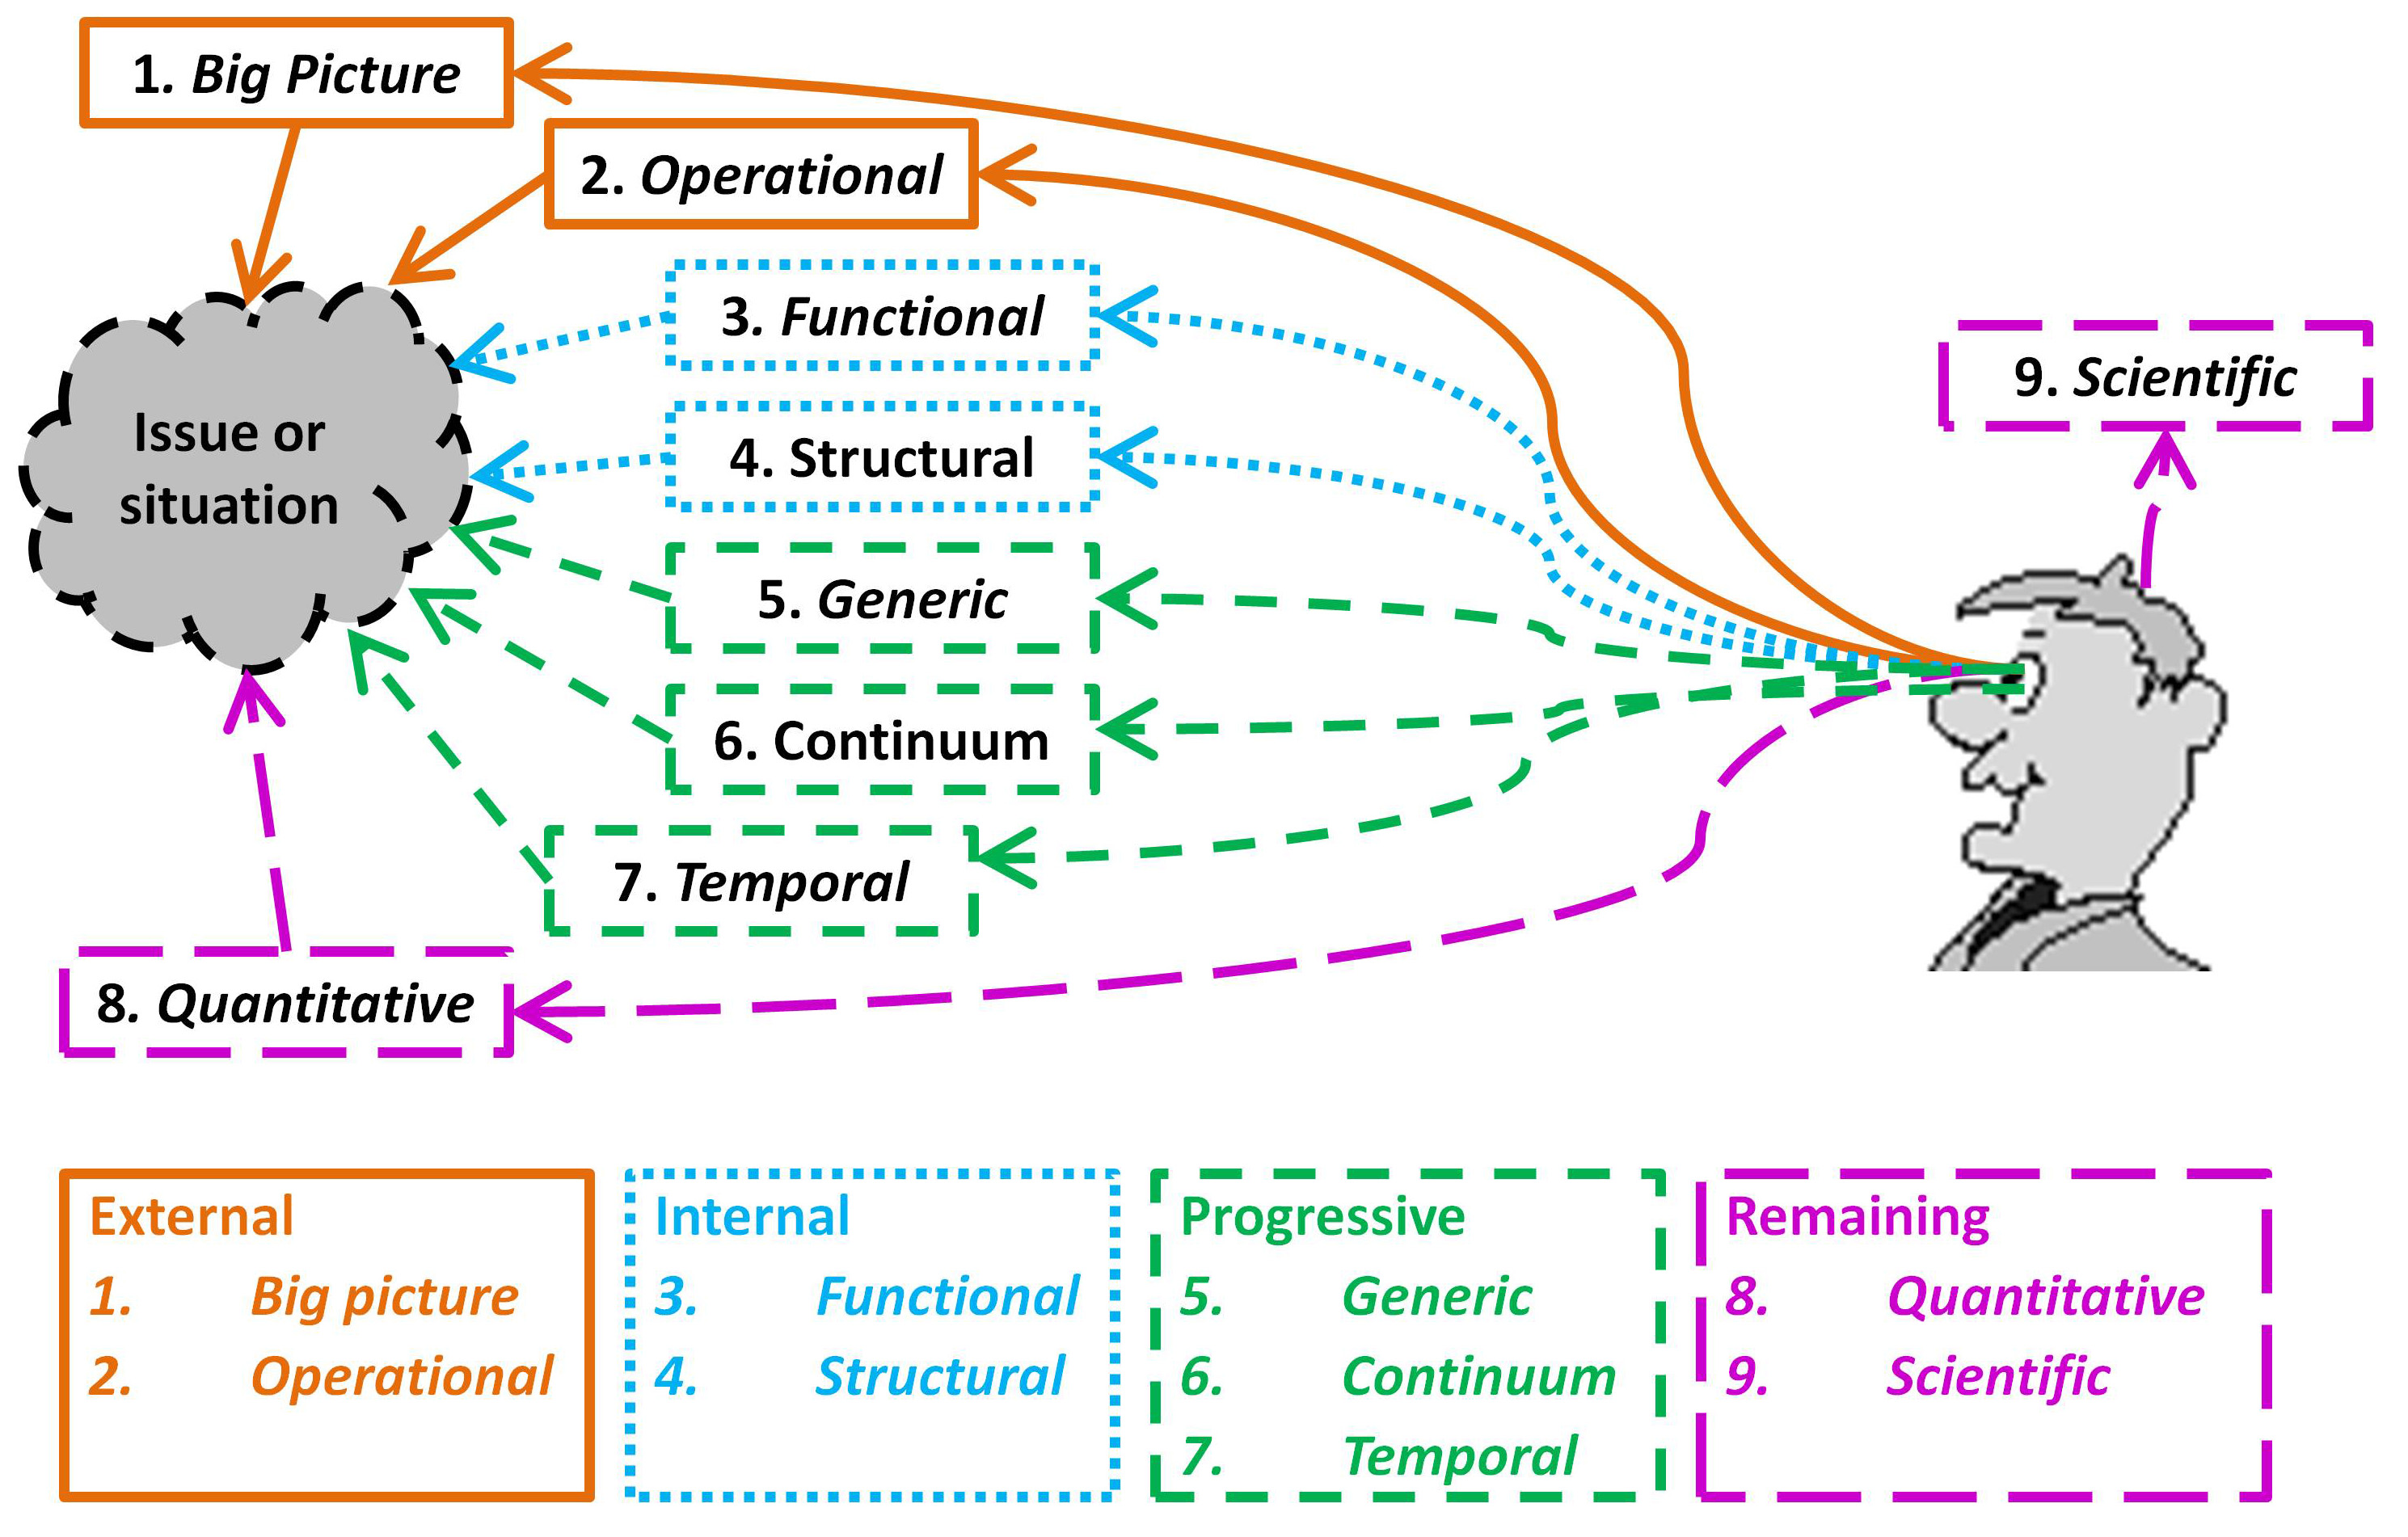
\includegraphics[height=0.3\textheight]{res-ch2/HTPs.jpg}
    \caption[Holistic thinking overview]{Overview on Holistic Thinking \cite{kasser_2018}}
\end{figure}

\subsubsection{Design Thinking}

In this design process publicized in 2005 by British Design Council, emphasizes on exploring issues (problem and solution) wide and deep (also known as divergent thinking), while taking focused action (also known as convergent thinking). \cite{banathy_1996, BDC_2005}

\begin{figure}[!h]
    \centering
    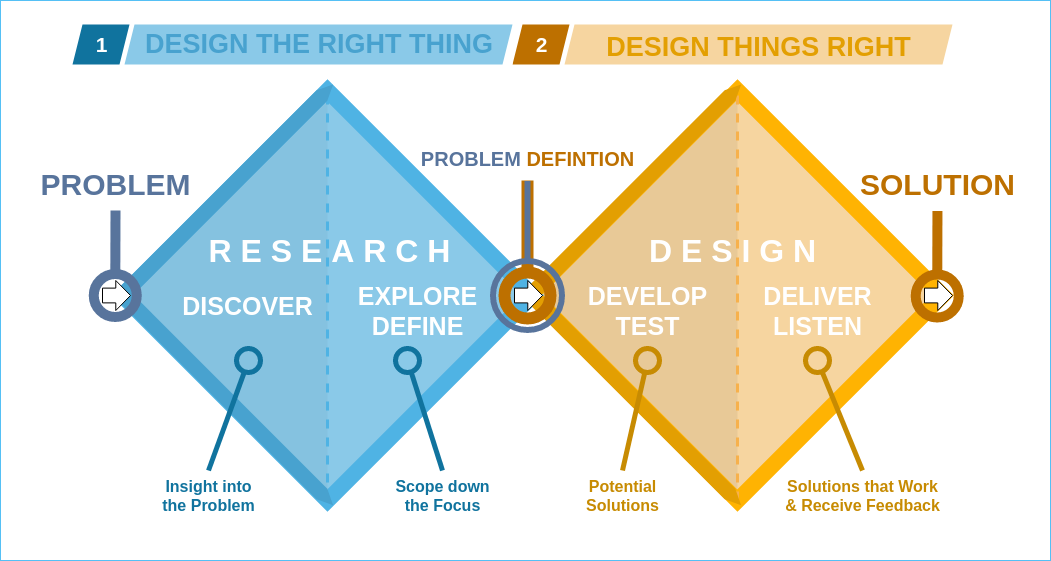
\includegraphics[height=0.3\textheight]{res-ch2/Double_diamond.png}
    \caption{Double diamond design}
\end{figure}

\clearpage